\Chapter{PERFORMANCE SIGNATURE APPROACH}\label{sec:Approach}

This chapter presents the method we introduce to determine the model that is closest to the ground truth for a given data set.  We refer to this method as ``Performance Signature'' approach, or ``Signature'' approach for short. 

The basic principles of the method is to define a vector space of model performances, namely the models described in chapter \ref{sec:RevLitt}.  Then, synthetic data is created with each model, and each model's performances are measured over each of the synthetic data set.  These measures represent a point in that space which is called \textbf{Performance prototype}. The synthetic data point associated with that point represents the ground truth prototype, or the centroid for classification.  Given a new data set, a \textbf{Target Performance Vector} can be obtained. Then, we use a nearest neighbor approach with a correlation distance to identify the closest ground truth model.

Let us rephrase the method in more specific terms and consider a set of models, $\mathcal{M}$, and a vector~$\mathbf{p}$ of length~$|\mathcal{M}|$ that contains the performance of each model over a given data set.  This \textbf{Target Performance Vector} represents a point in the performance space.  For each model $M \in \mathcal{M}$, we determine a \textbf{Performance prototype} point in the performance space that corresponds to synthetic data generated with model~$M$.  Then, for a given data set, we find the nearest synthetic data set point, using correlation as a distance, and consider the model behind it to be the ground truth.


The rest of the chapter goes into more details about the method.

\section{Model fit in a vector space framework}

The performance data in table~\ref{tab:vectorspace} will serve here to explain the method with a concrete example.  In this table, the predictive accuracy of the 6~models reviewed in chapter~\ref{sec:RevLitt} is reported against 6~synthetic data sets generated with the same models.  A seventh ``model'' named \textit{expected} (section~\ref{sec:basel-expect-pred}) and a seventh data set named \textit{random} (random results that constrained to reflect the target data set parameters such as item and student success rate distribution) are added for comparison purpose.  

\newcolumntype{d}[1]{D{.}{.}{#1}} % not used

\begin{table}[ht]
\caption{Vector space of accuracy performances}\label{tab:vectorspace}
\centering
\begin{tabular}{lccccccc}
  \toprule
  \multicolumn{1}{c}{\multirow{2}{*}{\textbf{Model}}} & \multicolumn{7}{c}{\textbf{Synthetic data set }\tablefootnote{Note that the Synthetic datasets are generated based on different models. Namely, IRT means that the ground truth of the generated dataset assumed to be IRT model}} \\
  \cline{2-8}
  & \multicolumn{1}{c}{{\textit{Random}}} & \multicolumn{1}{c}{{POKS}} & \multicolumn{1}{c}{{IRT}} & \multicolumn{1}{c}{{DINA}} & \multicolumn{1}{c}{{DINO}} & \multicolumn{1}{c}{{Linear .Conj}} & \multicolumn{1}{c}{{Linear .Comp}} \\ 
  \hline
  \textit{Expected} & \textbf{0.75} & 0.91 & 0.90 & 0.72 & 0.72 & 0.78 & 0.93 \\ 
  POKS & 0.75 & \textbf{0.94} & 0.94 & 0.81 & 0.81 & 0.90 & 0.94 \\ 
  IRT & 0.75 & 0.91 & \textbf{0.95} & 0.73 & 0.73 & 0.79 & 0.89 \\ 
  DINA & 0.75 & 0.77 & 0.81 & \textbf{1.00} & 0.65 & \textbf{0.98} & 0.89 \\ 
  DINO & 0.75 & 0.63 & 0.56 & 0.66 & \textbf{1.00} & 0.68 & 0.91 \\ 
  NMF.Conj & 0.75& 0.59 & 0.53 & 0.95 & 0.65 & 0.97 & 0.58 \\ 
  NMF.Comp & 0.75 & 0.76 & 0.79 & 0.59 & 0.93 & 0.70 & \textbf{0.98} \\ 
  \bottomrule
\end{tabular}
\end{table}


As we can expect, the diagonal (in bold face, except for one, corresponding to the match between the underlying synthetic model and the model performance) generally displays the best performance since it corresponds to the alignment of the model and the ground truth behind the data.  This confirms the intuition behind the usual strategy of assuming the best performer is the model behind the ground truth.  However, this is not always the case. In this particular example, the DINA model show a better performance over the Linear Conj.\ data set, whereas this data set's corresponding model is the NMF Conj. 

The principle of the proposed approach is to use the whole column of performance as a vector to determine the closest model to the ground truth.  In that respect, if columns are considered as vectors in the space of dimensions created by model performances, we can use a similarity measure to determine the closest ground truth (or a distance measure if we consider the columns as a point in space).

The advantage of this approach is that it does not rely on a single performance value to determine the goodness of fit, but instead on a set of performances over different models.  The hypothesis is that this set of performances provides a more reliable measure of the goodness of fit of a set of models.  In turn, we assume that this measure is more likely to indicate which model will perform better in general, as opposed to which models performs the best in the case of the single data set at hand.

The approach can be considered as a means to avoid a kind of local minimum, considering the best performer as a good indicator of the ground truth, but not a perfect one. Indeed, table~\ref{tab:vectorspace} suggests that aligning the model with the ground truth does yield the best performance except for one case, but we will show more examples later that there are exeptions and that the proposed approach is better able to avoid these exceptions that would lead to a wrong conclusion if we were to rely on the best performer approach.

\section{Research questions}

Let us get back to the research questions and design implementation of experiments to answer them, This section explains a general framework for each experiment, later in chapter \ref{sec:SIGNATURE} the results of these experiment with more details are given. To make it straightforward we break the contribution into four experiments:

\begin{enumerate}
\item What is the \textit{performance vector} of student skills assessment models over real and over synthetic data created using the same models?
\begin{itemize}
\item Experiment 1: Predictive performance of models over real and synthetic data sets: In a first experiment, we focus on showing the performance of all models described in chapter \ref{sec:RevLitt} over synthetic and real data sets.  It provides an overview of the predictive performance of each model across the different synthetic and real datasets. The output of this experiment is the \textbf{Performance vector} or the \textbf{Performance signature} of a dataset.
\end{itemize}
\item Is the \textit{performance vector} unique to each synthetic data type (data from the same ground truth model)?
\begin{itemize}
\item Experiment 2: Sensitivity of the signature over different data specific parameters: This section tests the uniqueness of the Performance signature across different data generation parameters.
\end{itemize}
\item Can the \textit{performance vector} be used to define a method to reliably identify the ground truth behind the synthetic data?
\begin{itemize}
\item Experiment 3: Model selection based on \textit{performance vector} classification: This part proposes a framework for model selection as well as a measure that represents a measure for the goodness of fit of a model by comparing the target \textit{performance vector} of a real dataset and the performance prototype vectors obtained from each synthetic datasets.
\end{itemize}
\item How does the method compare with the standard practice of using the model with the best performance?  In particular, does the ground truth model identified better generalize over a space of parameter values?
\begin{itemize}
\item Experiment 4: Generality of the signature approach under different assumptions about the data: In a last experiment, we test the generality of the approach by classifying data sets with different data specific parameters in the \textit{performance vector} space. To validate the approach, we need to rely on synthetic data for which we know the underlying ground truth model.  A matrix is created with data sets generated from the different models, and each model performance is measured through a cross validation process (using experiment 1). This matrix allows us to classify a data set of unknown ground truth according to a nearest neighbor approach (using experiment 3). In fact, this experiment tests if the signature approach remains reliable on different conditions of parameters. And also it compares the accuracy of the classification between signature approach and the best performer approach. 
\end{itemize}
\end{enumerate}

\subsection{Experiment 1: Predictive performance of models over real and synthetic data sets}

The performance of each model is assessed on the basis of 10-folds cross-validation.  The training set is used to estimate model parameters that are later used in for the test set. For each test set, a model is fed with a set of item outcomes of a student, called the observed set, and the remaining items are the predicted, or inferred ones. The breakdown of the data for cross-validation is illustrated in figure~\ref{figMethod}. We fixed the number of observed items for each run on each data set. The minimum number of observed items is 9 and the maximum number is one item less than total number of items. 

\begin{figure}[h]
\centering
{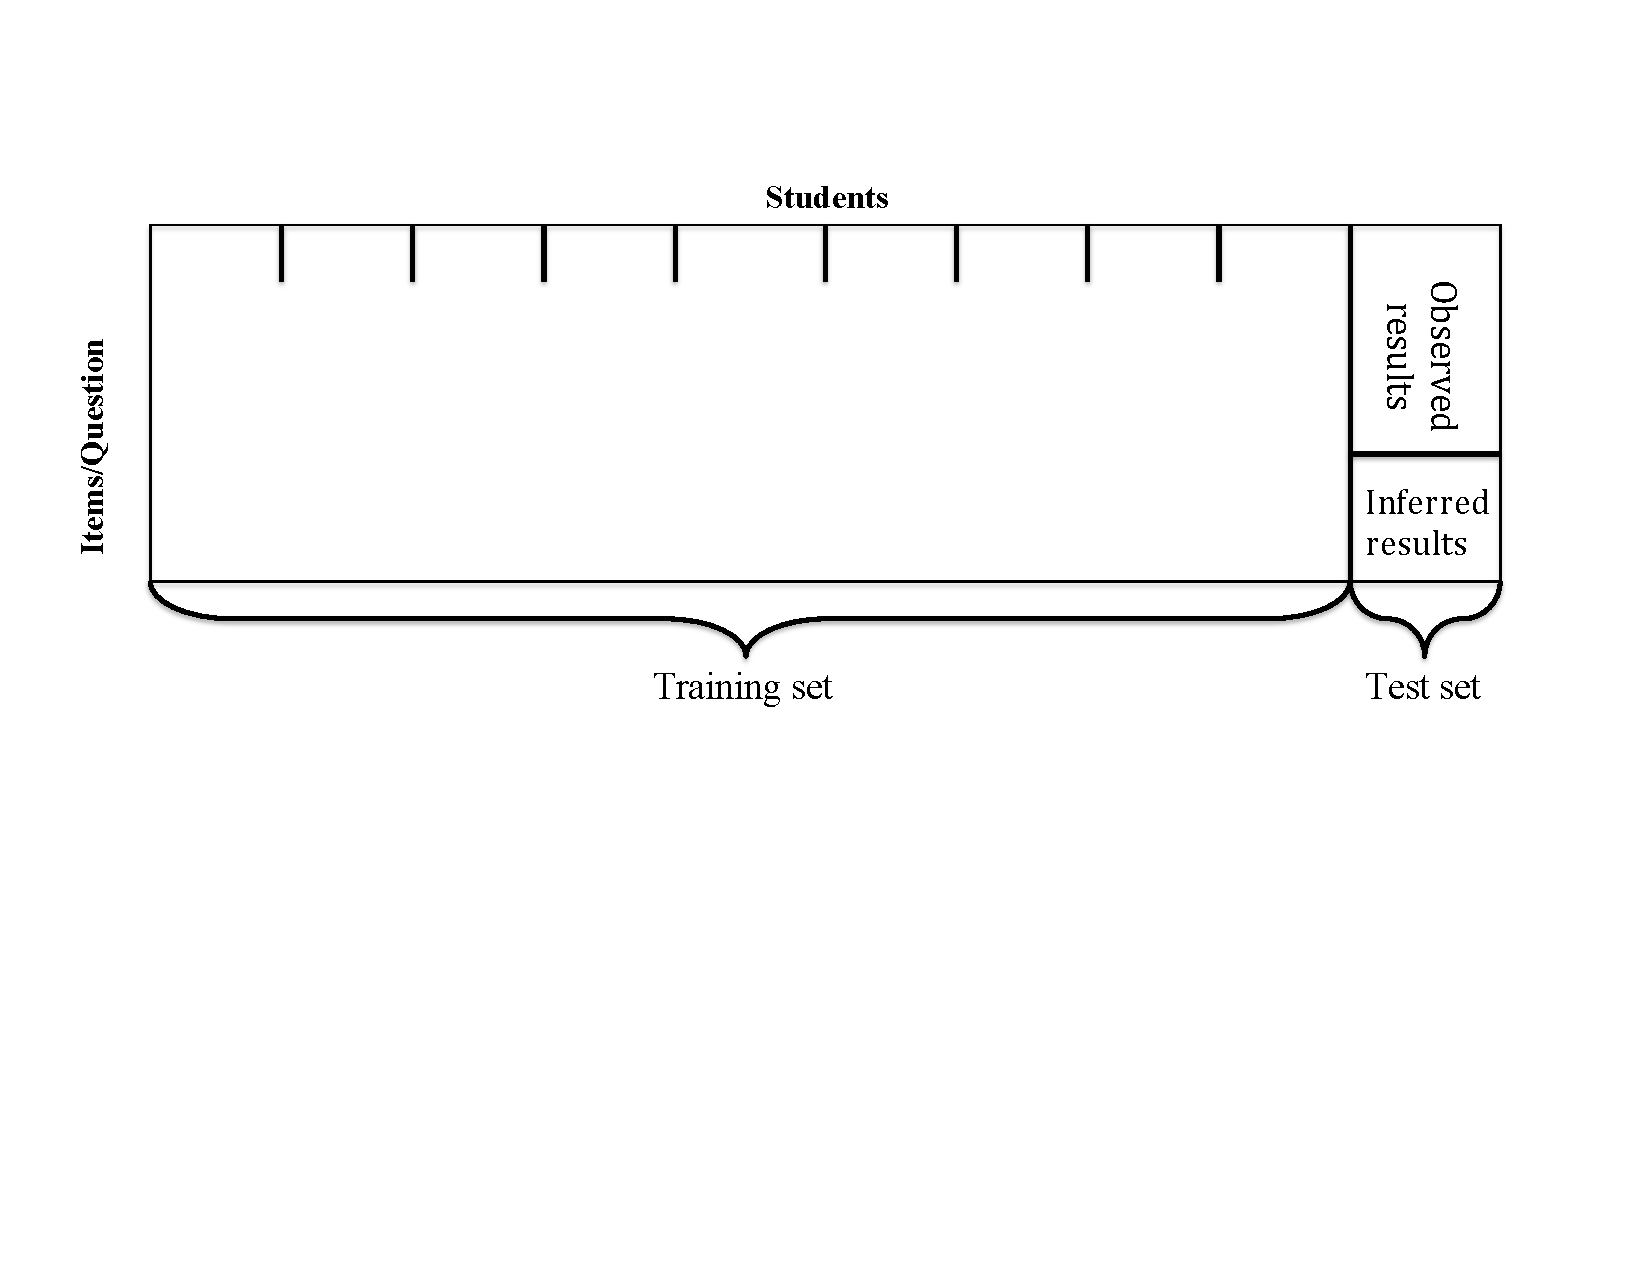
\includegraphics[trim=1cm 9cm 2.4cm 2.4cm,clip=true,width=.7\textwidth]{images/Methodology.pdf}}
\caption{Data breakdown of cross validation process}
\label{figMethod}
\end{figure}

For each dataset there exists a training set that contains 9 folds and a test set which represents a single fold. Samples are assigned randomly to each fold and this setting is the same across all predictive models for each run. Since all items are presented in the training set, then we can estimate the parameters that are related to items to be used in the test set. 

For other parameters that are related to students we need to divide the test set into an observed and inferred set. From the observed set we can get to the parameters that are related to students. A list of required model specific parameters for assessing the model performance is presented in table~\ref{fig:param-Predictive-Performance} \footnote{Details of all parameters are given in chapter \ref{sec:Syn}}.

\newcommand{\tabitem}{~~\llap{\textbullet}~~}
\newcommand\VRule[1][\arrayrulewidth]{\vrule width #1}

\begin{table}[h]
  \centering

\begin{tabular}{c|c|l!{\VRule[1.5pt]}l|l!{\VRule[1.5pt]}l|}
\multicolumn{3}{c}{}&\multicolumn{3}{c}{Parameters estimated from}\tabularnewline
\cline{4-6}
\multicolumn{3}{c!{\VRule[1.5pt]}}{Skills Model}&\multicolumn{2}{c!{\VRule[1.5pt]}}{Training set}&Observed items\tabularnewline
\cmidrule[1.5pt]{2-6}
&&NMF Conj. & & &  \tabularnewline
\cline{3-3}
&&NMF Add.&&& \tabularnewline
\cline{3-4}
&&DINA& \tabitem Slip & &\tabularnewline
\cline{3-3} 
&\multirow{-4}{*}{\begin{sideways} \scriptsize Multiple\end{sideways}}&DINO& \tabitem Guess&\multirow{-4}{*}{ \tabitem  Q-matrix }&\multirow{-4}{*}{  \parbox[t]{3cm}{ \tabitem Students skills  \\ mastery matrix}} \tabularnewline
\cmidrule[1.5pt]{2-6}
&&&\multicolumn{2}{l!{\VRule[1.5pt]}}{\tabitem Item difficulty  } &  \tabularnewline
&&\multirow{-2}{*}{ IRT}&\multicolumn{2}{l!{\VRule[1.5pt]}}{\tabitem Item discrimination}  &\multirow{-2}{*}{\tabitem Student Ability} \tabularnewline
\cline{3-6}
&\multirow{-3}{*}{\begin{sideways} \scriptsize Single \end{sideways}}&Expected&\multicolumn{2}{l!{\VRule[1.5pt]}}{\tabitem Item Odds}  &\tabitem Student Odds \tabularnewline
\cmidrule[1.5pt]{2-6}
&&&\multicolumn{2}{l!{\VRule[1.5pt]}}{\tabitem Initial Odds } & \tabularnewline
&&&\multicolumn{2}{l!{\VRule[1.5pt]}}{ \tabitem Odds ratio } & \tabularnewline
\multirow{-9}{*}{\begin{sideways} \scriptsize Contributed skills \end{sideways}}&\multirow{-3}{*}{\begin{sideways} \scriptsize Zero\end{sideways}}&\multirow{-3}{*}{ POKS }&\multicolumn{2}{l!{\VRule[1.5pt]}}{\tabitem Partial order structure}&\multirow{-3}{*}{ }\tabularnewline
\cmidrule[1.5pt]{2-6}
\end{tabular}
  \caption{Parameters of the predictive performance framework}
  \label{fig:param-Predictive-Performance}
\end{table}

Once all the required parameters are presented we can make a prediction for the inferred cells of the result matrix. Note that the selected observed and inferred items are the same across all the models for each run to make a better comparison for their prediction. A probability of mastery is obtained and rounded, resulting in a 0/1 error loss function.  We report the mean accuracy as the performance measure later in chapter \ref{sec:SIGNATURE}.  The R package \texttt{ltm} is used for parameter and skills estimation for IRT model and the R package \texttt{CDM} and \texttt{NMF} for Deterministic Input Noisy and NMF models. 

\note{This is a description of experiments whose results are presented one chapter later.  Not ideal, but I understand it is also necessary to introduce the data generation chapter.  We may leave it as is, but I add this note for the moment}

\subsection{Experiment 2: Sensitivity of the Model performance over data generation parameters}
\label{Sensitive}

In this experiment we want to examine the effect of data specific parameters on the stability of the performance prototype vector in the performance space. We run the same experiment as before but with different contextual data generation parameters such as average success rate, sample size, number of latent skills, number of items, student and item score variance. This experiment can answer the question whether the pattern of performance signatures for datasets with the same ground truth remain stable across different conditions. Also it can answer whether the synthetic datasets to assess model fit should follow the same data specific parameters as the real data.


\subsection{Experiment 3: Model selection based on \textit{performance vector} classification}
\label{Sigapproach-measure}
This experiment essentially introduces the ``signature'' approach. By the assumption that previous experiment proves that the uniqueness characteristic of synthetic data signatures makes it easy to identify the ground truth and also there exists some similarity between the pattern of performance signature of synthetic and real datasets (chapter \ref{sec:SIGNATURE} explains these results). Hence we can define a measure for the similarity of a synthetic generated dataset and a real one given a set of candidate models. Given that our objective is to determine the ground truth of a given data set, we will borrow data specific parameters from this data set to generate the synthetic data.  Further details on data generation are given in chapter~\ref{sec:Syn}. 

As explained before, signature approach search for the nearest neighbor of the target \textit{performance vector} among the performance prototypes. The principal of this search is to find the closest performance prototype to the target \textit{performance vector} in the performance space. Since this search is in a hyper space we used a linear discriminant approach which is the nearest neighbor classifier. This approach essentially splits the space into parts with a defined surfaces. However there exists other approaches to define a surface such as SVM \citep{cortes1995support}, single layer neural network \citep{lippmann1987introduction} or LDA \citep{blei2003latent}. We do not directly define any surface in the performance space but we just measure the closest neighbor. In this experiment we used Pearson correlation coefficient as a measure of similarity to find the nearest neighbor.

There are two approaches to search for the nearest neighbor in this space:
\begin{itemize}
\item Centroid performance prototype: In total there are $7$ neighbors(points in performance space) for this search where each of them is a representative of a performance prototype of a skills assessment ground truth (Chapter \ref{sec:RevLitt} explains these models in details). Each centroid performance prototype is defined as the average of \textit{performance vectors} of $10$ datasets generated with the same model and data specific parameters but different seeding points. The nearest neighbor among these $7$ centroid \textit{performance vectors} becomes the estimated ground truth.
\item Majority voting among $10$ nearest neighbors: This approach considers all neighbors in the search without defining a centroid point for each performance prototype. In this case the distance between each neighbor's \textit{performance vector} and the target \textit{performance vector} is calculated and a majority voting among the ground truth of $10$ nearest neighbors defines the estimated ground truth.
\end{itemize}

In this experiment we used the first approach to define the closest neighbor. However, both approaches show identical results.


%\subsubsection{Methodology and degree of similarity}

%\note{Can we do away with this section?  This is a description of the basic principles that were already described, no?  The only difference is that we specify which parameters are taken from the target data (the data set to classify).  If so, then we may want to have a section that describes only this, not the whole process since it becomes confusing to understand whether this is the same process described earlier or some variant.}

%The methodology that we took to assess the goodness of fit for a dataset is straightforward. It contains few steps as following:
%\begin{itemize}
%\item Obtaining the parameters of the given data: This step extracts the two types of parameters of the real data which are model and data specific parameters. 
%\item Generating synthetic datasets with the obtained parameters based on each candidate models: In our study we took 7 candidate models. Since some parameters influence the \textit{performance vector} as we will see later in chapter~\ref{sec:SIGNATURE} so we have to create synthetic data that follows the same characteristics of the real one.

%\item Calculating the predictive performance of candidate models over both real and synthetic datasets: This process will result in eight signatures where only one of them is for the given real data.
%\item Measuring the similarity of the signature derived from real and each synthetic data: Each predictive performance in the previous step will become a point in the performance space. the predictive performance point for a synthetic data is in the area of the relative ground truth. Therefore the nearest neighbor to the real data performance in the performance space will become the best representative of the ground truth. In this research we used Pearson correlation coefficient as a measure of similarity to find the nearest neighbor.
%\end{itemize}


%\item Experiment 4: Generality of the signature approach under different assumptions about the data: In a last experiment, we test the generality of the approach by classifying data sets with different data specific parameters in the \textit{performance vector} space. To validate the approach, we need to rely on synthetic data for which we know the underlying ground truth model.  A matrix is created with data sets generated from the different models, and each model performance is measured through a cross validation process (using experiment 1). This matrix allows us to classify a data set of unknown ground truth according to a nearest neighbor approach (using experiment 3). In fact, this experiment tests if the signature approach remains reliable on different conditions of parameters. And also it compares the accuracy of the classification between signature approach and the best performer approach. 

\subsection{Experiment 4:  Generality of the signature approach under different assumptions about the data}
\label{Classification}

The very last experiment is to test the generality of signature approach to assess a model fit over different data specific parameters. Despite the fact that different data specific parameters may affect the performance signature (as we will see in the results of experiment 2), this experiment tests the reliability of this approach to estimation of the ground truth on different assumptions about the data. Akin to experiment 2, this experiments relies on synthetic datasets since the ground truth and data specific parameters are known. 

Considering $6$ data specific parameters which are presented in table \ref{fig:param-Predictive-Performance} and $4$ different values for each parameter, while others have default values, results in $24$ different conditions for the data generation process. The goal of this experiment is to obtain the accuracy of signature approach to classify any dataset with each of these $24$ conditions. Therefore, with each condition we generate $10$ datasets with different seeding point for each skills assessment ground truths. This results in $60$ datasets for each condition. let us name this set of $60$ datasets as a \textbf{group}. Totally $24$ \textbf{groups} can be generated.

The classification is preforming among the members of a \textbf{group} where all datasets share the same data specific parameters. We randomly select a dataset whose \textit{performance vector} becomes the target \textit{performance vector}. Consequently the other $59$ datasets in the \textbf{group} are neighbors with performance prototype vectors. As explained in experiment 3 we can calculate the distance between the target \textit{performance vector} and each of neighbors for the purpose of model selection. Finally a majority voting among the ground truth of 10 nearest neighbors defines the ground truth. This process repeats for each \textbf{group}.

Obviously the highest performance in a \textit{performance vector} is the classification result for the ``best performer'' approach. Later in section\ref{GeneralityRes} we use the classification measures from section \ref{MeasuresT} to compare the reliability of these two approaches.
